\section{Context Engine}
\label{sec:design:context-engine}

The following section suggests a design of the engine used to recognize the context the user is situated in and ultimately choosing an appropriate action to trigger in the recognized context. The design is suggested based on the requirements presented in \Cref{sec:analysis:context-engine}.

The context engine consists of the following two things.

\begin{itemize}
\item One or more context providers.
\item The context recognizer.
\end{itemize}

The context providers supply information about a specific part of the environment. Examples of context providers include the position context provider and the gesture context provider. The providers suggest a set of actions that are valid in the part of the context it knows about and assigns a probability to those actions.

Consider the following example of how the gesture context provider supplies its information about the context.

\begin{testexample}
A user is equipped with a wearable and performs a gesture. The gesture recognizer utilizes the accelerometer to recognize categorize the motion performed by the user. As a result the recognizer suggests a set of gestures. For each gesture the recognizer assigns a score indicating the similarity between the gesture and the motion performed by the user.
For each gesture in the set we find the actions associated with the gesture. The scores are converted to probabilities and the probabilities are assigned to the actions and normalized.
The context provider supplies these actions and the probability as \textit{outcomes} indicating the likelihood that the user desired to trigger the action.
\end{testexample}

In the above example, actions are suggested with a probability based on the motion performed by the user. Because the gesture context provider does not know anything aobut the environment but the set of gestures recognized by the gesture recognizer, it is the only information it can use to assign probabilities to the actions.

Consider the following example of how the position context provider can supply information about the context.

\begin{testexample}
A user is equipped with a wearable and walks around his room installed with Bluetooth LE beacons. As the user moves around, the position context provider determines the likelihood that the user is in each room. There may be fluctations in the readings, \ie~a reading indicating the the user is in a wrong room, so the provider continuously measures the position and adjusts the probabilities accordingly.
The probability in each room is directly converted to probabilities of each action that can be performed in the room. The probabilities are normalized.
\end{testexample}

In the above example, the position context provider only knows about the users position and suggests probabilities for each action that can be performed in the room. By combining the gesture context provider and position context provider, we can get a better understanding of the context and choose the correct action based on the joined probabilities. Note that it may make sense for the context providers to only include actions if there is a significant certainty that the action should be triggered. For example, we only consider gestures which has a score greater than a threshold as explained in \cref{} \todo[author=Simon]{Indsæt reference til beskrivelse af gesture recognition og threshold introduceret for ikke at inkludere gestures med lavt threshold}.

\Cref{fig:design:context-engine:single-suggestion} illustrates an example of the context engine configured with three context providers. In this case the context providers suggest a total of three actions, Action 1, Action 2 and Action 3. Actions with a zero probability is left out. The position context provider suggests all three actions, all with different probabilities. Since the context provider only knows about the position of the user, we can conclude that the user has visited three different rooms. The room in which Action 1 can be triggered was visited the latest and therefore it has the highest probability.

The gesture recognizer has found two gestures to be likely, however, the gesture associated with Action 1 has a significantly higher score than the gesture for Action 2.

The system state provider supplies probabilities for all actions that it currently makes sense to trigger in the system. It makes sense to trigger Action 1 and Action 3. It could be that Action 2 turns on a light which is already turned on, therefore it does not make sense to trigger it and it has a probability of zero. The total probability is distributed among all actions it makes sense to trigger. Therefore the system state provider can be regarded as a \textit{filter}, as it only filters out actions.

In \cref{fig:design:context-engine:single-suggestion} the probabilities of actions are represented by a line from the action, \ie~a circle, to the probability. The identifiers of each action is written inside the circle. 

Context providers are assigned a weight, shown below the name of the context provider in \cref{fig:design:context-engine:single-suggestion}. Weights are introduced in order ​to​ model precedence and reduce the risk of triggering the wrong action. This could happen if the position context provider assigns a high probability to an action that the gesture context provider assigns a low probability to. By introducing weights we can make the gesture recognizer more significant than other recognizes and reduce the risk that we trigger an action which the gesture context provider assigned a low probability.

The context recognizer takes all the context providers as input and outputs an appropriate action to be triggered. The context recognizer calculates the probability of an action $a$ as shown in the equation below where $p_a$ is the total probability of the action, $CP$ is the set of context providers, $p_{a,x}$ is the probability of action $a$ in set $x$ and $w_x$ is the weight of set $x$.

\begin{equation*}
p_a = \sum\limits_{x \in CP}^{} p_{a,x} \cdot w_{x}
\end{equation*}

The action with the highest probability, \ie~the highest $p_a$, is suggested by the context recognizer.

\begin{figure}[h!]
\centering
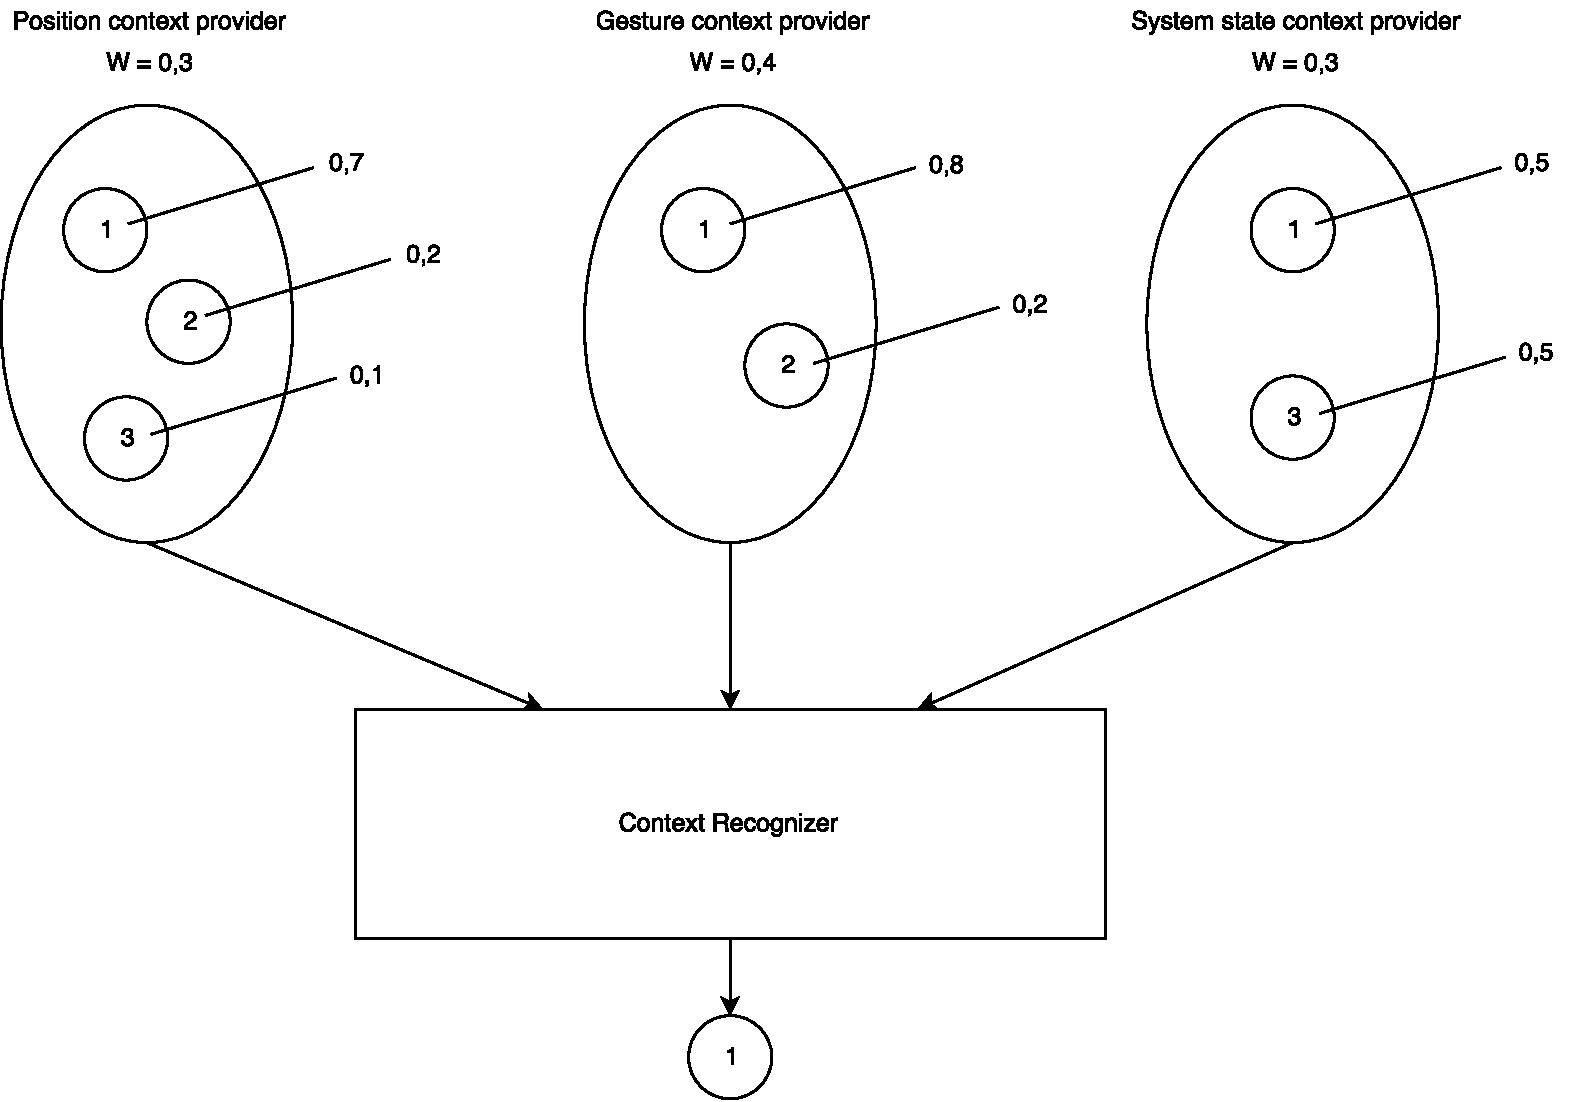
\includegraphics[width=0.75\textwidth]{images/context-engine-single-suggestion}
\caption{Example of a context engine configured with three providers. The recognizer suggests a single action. Ovals represent context provider and circles present actions. Each action is assigned a probability, represented by a line from the action to the probability.}
\label{fig:design:context-engine:single-suggestion}
\end{figure}

As illustrated in \cref{fig:design:context-engine:multiple-suggestions}, the context engine can suggest multiple actions if the probablities are the same as it is the case for actions 1 and 2. In this case both action should be suggested to the user and the user should choose whcih action to be triggered.

Another threshold can be introduced to the calculated probability in order to suggest actions that are almost equally likely to be triggered. If, for example, the context recognizer calculates Action 1 to have a probability of 80\% and Action 2 to have a probability of 79\%, this may be an insignificant basis to suggest Action 1 over Action 2 and therefore both actions should be suggested.

\begin{figure}[h!]
\centering
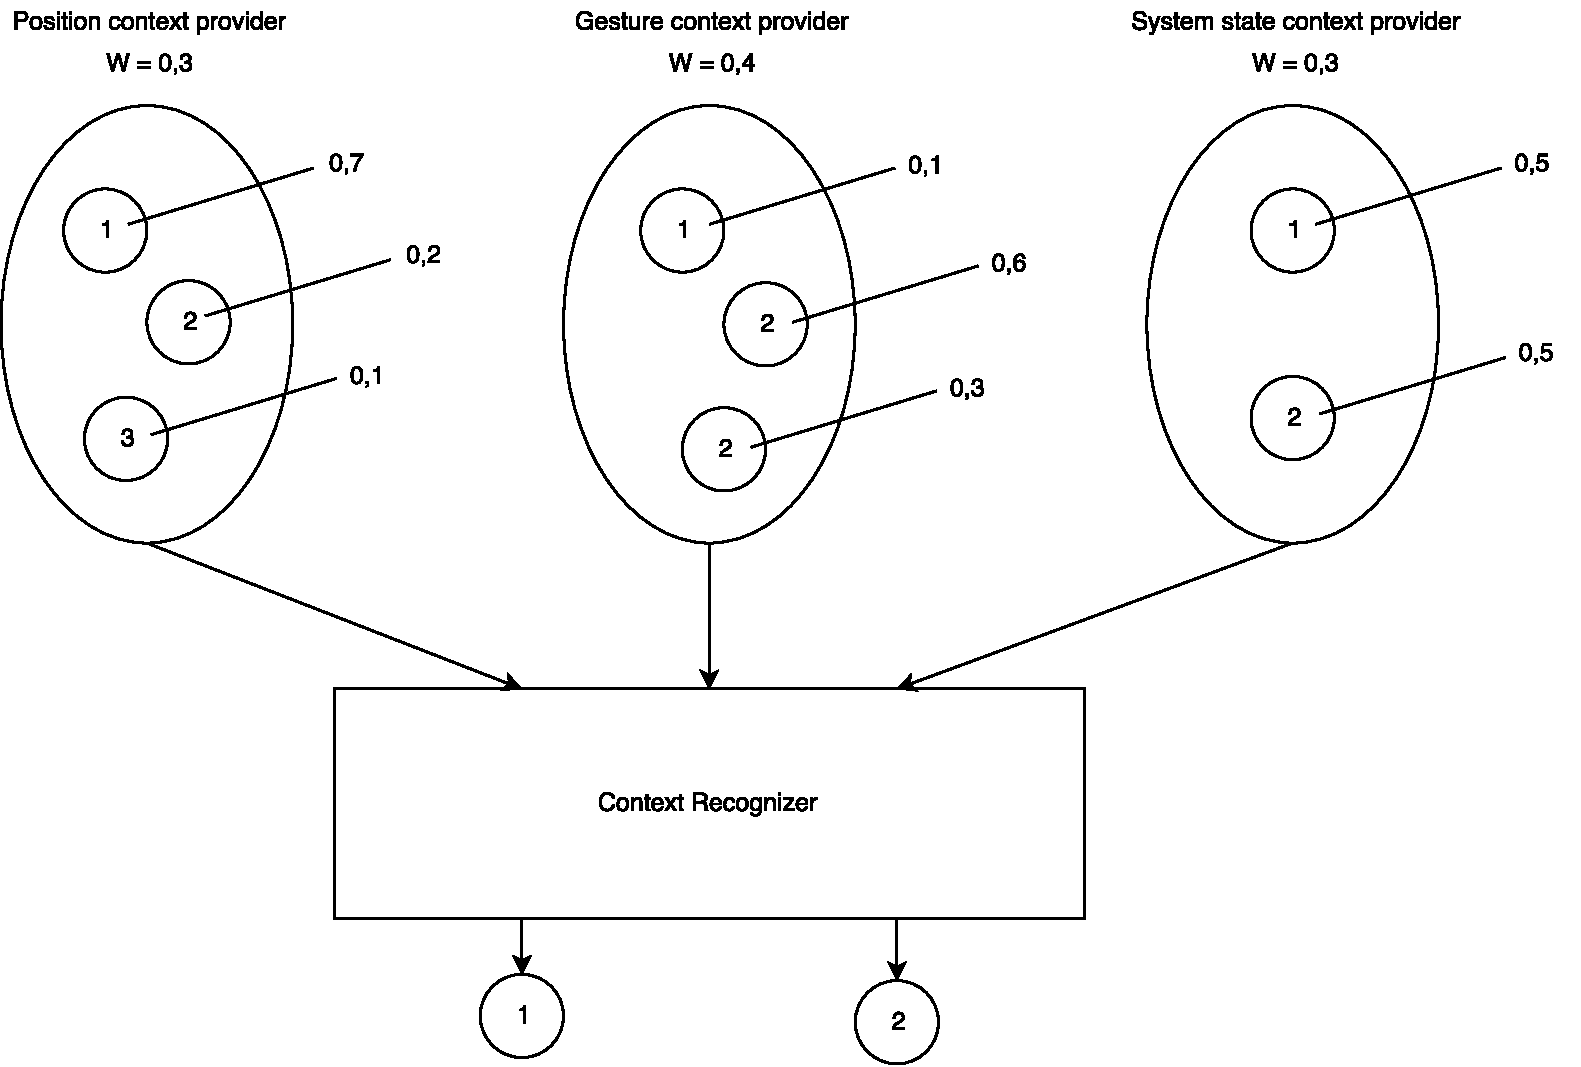
\includegraphics[width=0.75\textwidth]{images/context-engine-multiple-suggestions}
\caption{Example of a context engine configured with three providers. The recognizer suggests multiple actions. Each action is assigned a probability, represented by a line from the action to the probability.}
\label{fig:design:context-engine:multiple-suggestions}
\end{figure}

\subsection{Starting Context Recognition}
\label{sec:design:context-engine:starting-contxt-recognition}

In theory, the context engine can be started at any time. We start the engine when the gesture recognizer recognizes one or more candidate gestures. The gestures are supplied to the gesture context provider as described in \cref{sec:design:gesture-context-provider}.

When the engine is started, it will ask all registered context providers to supply information about the context. The gesture context provider will calculate probabilities of actions as described in \cref{sec:design:gesture-context-provider} and supply them to the context recognizer.

The context providers should supply their information within a specified interval, \eg~two seconds, and if they do not respond within the interval, they will be cancelled and not considered in the final calculations. This is to ensure a minimum delay between starting the context engine, choosing an action and triggering that action.

\subsection{Class Diagram}
\label{sec:design:context-engine:class-diagram}

\Cref{fig:design:context-engine:class-diagram} shows the class diagram for all classes and interfaces involved in the context engine. Below is a short description of each component.

\begin{description}
\item[ContextProvider] Objects implementing the interface provides information about a part of the context. Examples of this include the position context provider described in \cref{sec:design:position-context-provider} and the gesture context provider described in \cref{sec:design:gesture-context-provider}.
\item[ContextProviderListener] Objects implementing the interface and which are registered with a context provider are informed when a context provider has information about the context ready or when it fails.
\item[ContextRecognizer] The recognizer has a set of context providers and asks those to provide information about the context when the recognizer is started. Based on the retrieved information it determines the appropriate action to trigger of suggests multiple actions.
\item[ContextRecognizerListener] Objects implementing the interface and which are registered with the context recognizer are informed when the recognizer has recognized the context, fails recognizing the context or the recognition times out. A time out may occur if the recognizer does not get information from the providers within a certain interval.
\item[ContextOutcome] Context providers supply outcomes to the context recognizer. An outcome represents an action by the ID of the action and contains a probability. The context recognizer returns the outcomes when the context has been recognized.
\end{description}

\begin{figure}[h!]
\centering
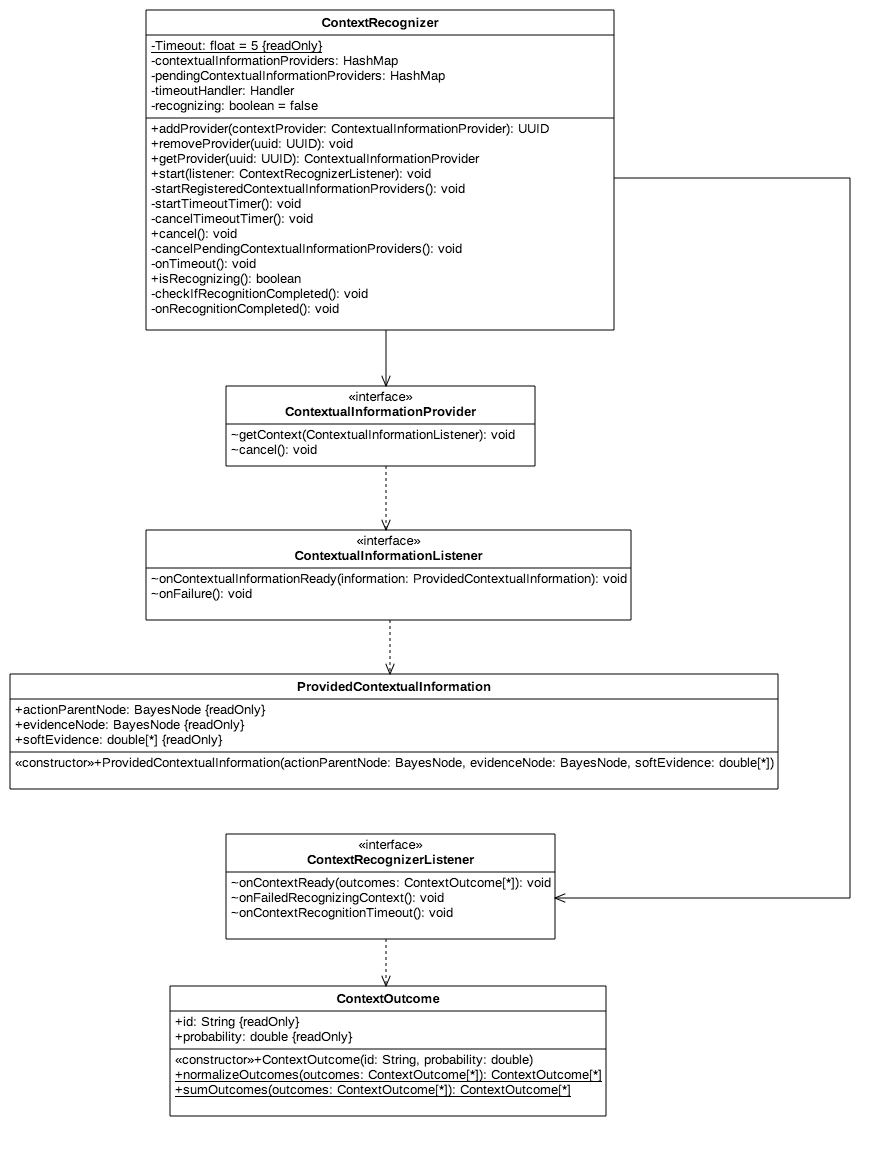
\includegraphics[width=\textwidth]{images/uml-context-engine}
\caption{Class diagram showing all classes and interfaces involved in the context engine.}
\label{fig:design:context-engine:class-diagram}
\end{figure}

%%% Local Variables:
%%% mode: latex
%%% TeX-master: "../../master"
%%% End:
